\documentclass[authorversion,nonacm]{acmart}
%\documentclass[11pt]{article}
%\usepackage[margin=1in]{geometry}}
% set font to 11pt

%\usepackage[hashEnumerators,smartEllipses]{markdown}
\usepackage{pgfplots, pgfplotstable}
\usepackage{url}
\usepackage{tikz}
\usepackage{natbib}
\usepackage{float}
\usepackage{etoolbox}
\usepackage{caption}
\usepackage{subcaption}
\usepackage{listings}
\usepackage{lstautogobble}
\usepackage{xcolor}
\usepackage{balance}
\usepackage{tikz}
\usetikzlibrary{decorations.pathreplacing,calc,shapes,positioning,tikzmark, trees}
\pgfplotsset{compat=1.17}

\renewcommand{\boxed}[1]{\text{\fboxsep=.2em\fbox{#1}}}

\settopmatter{printacmref=false}

\definecolor{darksky}{rgb}{0.4,0.4,1}
\definecolor{skyblue}{rgb}{0.25,0.78,0.96}
\definecolor{lightyellow}{rgb}{1,0.96,0.52}
\definecolor{lightorange}{rgb}{1,0.7,0.4}
\definecolor{lightred}{rgb}{1,0.4,0.4}

\definecolor{codegreen}{rgb}{0,0.6,0}
\definecolor{codegray}{rgb}{0.5,0.5,0.5}
\definecolor{codepurple}{rgb}{0.58,0,0.82}
\definecolor{backcolour}{rgb}{0.95,0.95,0.92}

\lstdefinestyle{python}{
  backgroundcolor=\color{backcolour},   
  commentstyle=\color{codegreen},
  keywordstyle=\color{magenta},
  numberstyle=\tiny\color{codegray},
  stringstyle=\color{codepurple},
  basicstyle=\ttfamily\footnotesize,
  breakatwhitespace=false,         
  belowskip=-0.5em, breaklines=true,                 
  captionpos=b,                    
  keepspaces=true,                 
  numbersep=5pt,                  
  basicstyle=\footnotesize,
  showspaces=false,                
  showstringspaces=false,
  showtabs=false,                  
  tabsize=4
}

\lstset{style=python}

\usetikzlibrary{arrows}

%
%
%


\definecolor{rosso}{RGB}{220,57,18}
\definecolor{giallo}{RGB}{255,153,0}
\definecolor{blu}{RGB}{102,140,217}
\definecolor{verde}{RGB}{16,150,24}
\definecolor{viola}{RGB}{153,0,153}


\tikzset{
  chart/.style={
    legend label/.style={font={\scriptsize},anchor=west,align=left},
    legend box/.style={rectangle, draw, minimum size=15pt},
    axis/.style={black,semithick,->},
    axis label/.style={anchor=east,font={\tiny}},
  },
  pie chart/.style={
    chart,
    slice/.style={line cap=round, line join=round, very thick,draw=white},
    pie title/.style={font={\bfseries}},
    slice type/.style 2 args={
        ##1/.style={fill=##2},
        values of ##1/.style={}
    }
  }
}

\pgfdeclarelayer{background}
\pgfdeclarelayer{foreground}
\pgfsetlayers{background,main,foreground}


\newcommand{\pie}[3][]{
    \begin{scope}[#1]
    \pgfmathsetmacro{\curA}{90}
    \pgfmathsetmacro{\radius}{1}
    \def\Centre{(0,0)}
    \node[pie title] at (90:1.3) {#2};
    \foreach \v/\s in{#3}{
        \pgfmathsetmacro{\deltaA}{\v/100*360}
        \pgfmathsetmacro{\nextA}{\curA + \deltaA}
        \pgfmathsetmacro{\midA}{(\curA+\nextA)/2}

        \path[slice,\s] \Centre
            -- +(\curA:\radius)
            arc (\curA:\nextA:\radius)
            -- cycle;

   % to determine direction of lines (left/right, up/down
   \pgfmathsetmacro{\ysign}{ifthenelse(mod(\midA,360)<=180,1,-1)}
   \pgfmathsetmacro{\xsign}{ifthenelse(mod(\midA-90,360)<=180,-1,1)}

   \begin{pgfonlayer}{foreground}
        \draw[*-,thin] \Centre ++(\midA:\radius/1.1) -- 
                               ++(\xsign*0.1*\radius,\ysign*0.3*\radius) -- 
                               ++(\xsign*\radius,0) 
                      node[above,near end,pie values,values of \s]{$\v\%$};
   \end{pgfonlayer}


        \global\let\curA\nextA
    }
    \end{scope}
}

\newcommand{\legend}[2][]{
    \begin{scope}[#1]
    \path
        \foreach \n/\s in {#2}
            {
                  ++(0, -10pt) node[\s,legend box] {} +(5pt,0) node[legend label] {\n}
            }
    ;
    \end{scope}
}



%
%
%

\AtBeginDocument{%
  \providecommand\BibTeX{{%
\normalfont B\kern-0.5em{\scshape i\kern-0.25em b}\kern-0.8em\TeX}}}

%% These commands are for a PROCEEDINGS abstract or paper.

\begin{document}

%\definecolor{rosso}{RGB}{220,57,18}
%\definecolor{giallo}{RGB}{255,153,0}
%\definecolor{blu}{RGB}{102,140,217}
%\definecolor{verde}{RGB}{16,150,24}
%\definecolor{viola}{RGB}{153,0,153}


\title{Informing the Design and Utilization of Distractors in Parsons Problems}

\author{David H. Smith IV}

%1-2 page intro  (why should I care?)
%2-3 pages background / related work  (have you done your homework?)
%4-5 pages on previous work  (are you ready to prelim?  will you be successful on future work?)
%4-5 pages on future work  (what are you proposing to do?  why?  how?)
%1 page on schedule  (is your schedule realistic?  will you have done enough to earn a Ph.D.?)

\begin{teaserfigure}
    \centering
    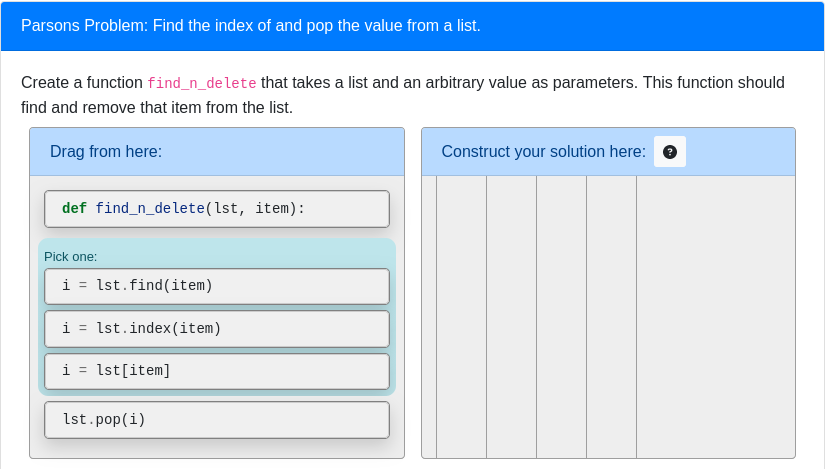
\includegraphics[width=0.70\textwidth]{imgs/parsons.png}
    \caption{Examples of Parsons Problems with Distractors on PrairieLearn}
\end{teaserfigure}

\maketitle

\section{Abstract}

% Very Brief intro to parsons problems.
Since their introduction by \citet{parsons2006parson} distractors have become
common place in studies investigating Parsons problems. However, to date, there
have been a limited number of studies investigating the utility of including
distractors in Parsons problems at all. In filling this gap, my work thus far
has focused on investigating methods of developing distractors and the impact
of distractors in Parsons problems in a summative context. I first introduce a
method of creating distractor templates from analysis of code writing errors
and using those templates to support the autogeneration of
distractors~\cite{smith2023discovering}. I am also currently in the process of
integrating this system of distractor autogeneration into the CodeSpec
platform~\cite{haynes2022codespec}. Since the creation of this tool, I have
conducted a series of studies comparing Parsons problems on exams that include
distractors to those that do not. These studies have also included a comparision
between different methods of including distractors, specifically comparing the
use of distractors that are jumbled amoungst the other options to distractors
that are visually grouped with their correct
alternative~\cite{smith2023investigating, smith2023comparing}.  In support of 
future work, I have also added the ability to associate feedback with distractors
in the PrairieLearn assessment platform. This enables investigations into the
impact of distractors in a formative context where ellucidating the reason a
distractor is incorrect may contribute to the learning process.


% My proposed future work
My proposed future work can be divide into three main areas of focus: (1)
performing further analysis of common errors made by students in code
writing exercises towards creating a taxonomy of distractors, (2) extending
my prior analysis investigating the impact of using distractors in summative
contexts, and (3) investigating the impacts of distractors in formative contexts.
In doing so, I hope to provide instructors and curriculum designers with a
better understanding of how distractors can be used in designing summative
assessments and learning activities alike.

\section{Introduction}

% What are parsons' + Distractors
Parsons problems were first proposed by \citet{parsons2006parson} as a method
of facilitating the development of fundamental semantic and syntactic concepts
in introductory programming students. These problems consist of individual
blocks of code that must be arranged in a specific order in order to construct
a valid solution. Code blocks that either contain errors or are not used in the
final solution, commonly referred to as distractors, were introduced in the
original and continue to be included in many studies involving Parsons
problems~\cite{du2020review}.  

% When are distractors used in Parsons and why?
Distractors are often design to reflect common programming errors and
misconceptions~\cite{du2020review, parsons2006parson}.  Much like with
multiple-choice questions, distractor blocks are added to Parsons problems with
the intention of distracting students with plausible, but incorrect
alternatives.  When included on homework assignments the purpose of distractors
is to illustrate and correct common errors and misconceptions students may have
when writing programs without having them deal with the full cognitive load of
writing a program from scratch~\cite{ericson2017solving, haynes2021problem}.
When included on exams, their purpose shifts to increasing the difficulty of the
base problem and providing an additional dimension by which to discriminate
based on student knowledge~\cite{smith2023discovering, smith2023investigating,
smith2023comparing}. As such, the selection of distractors that accurately
reflect common errors is important when pursuing either of these goals. 

% Where do distractors come from in the context of MC
The design and impact of distractors with respect to multiple-choice questions
has long been a topic of consideration given the widespread usage of this
question format.  As summarized by \citet{gierl2017developing}, designing
distractors is difficult for three main reasons. First, it requires an
experienced individual to write a large number of plausible but incorrect
options using either their own personal intuition or through the analysis of 
common errors made by students on related short response questions~\cite{briggs2006diagnostic,
halloun1985initial}. Next, if distractors are too obviously incorrect it can
limit the amount of thought students must put into answering the question. This,
in turn, may limits the learning potential of the
question~\cite{little2015optimizing}.  Finally, the quality of distractors
impacts the quality of feedback an instructor can receive from the question on
the misconceptions their class may hold.

% Research on distractors in Parsons problems in formative assessments
Compared to the large body of work investigating distractors in multiple-choice
questions, there is a relative dearth of work investigating distractors in
Parsons problems. The original intent of including distractors in Parsons
problems was to support students by illustrating and correcting common errors
in a scaffolded environment~\cite{parsons2006parson}. The limited work 
investigating the impact of distractors in Parsons problems has produced 
mixed results with some studies indicating that including distractors can
decrease learning efficiency~\cite{harms2016distractors} and others indicating
that practice distractors can improve student performance in subsequent 
code fixing exercises~\cite{ericson2023multi}.  Similarly, in the context of
summative assessments, there has been limited work investigating the impact of
including distractors in Parsons problems~\cite{denny2008evaluating}.

% Final paragraph on motivation for my work
Given the limited investigations into the impact of distractors in Parsons
problems, there is a need for further work investigating the impact of
distractors in both formative and summative contexts. My work aims to address
these gaps by investigating the impact of distractors in both formative and 
summative contexts. In the context of summative assessments, my work aims to 
provide instructors with a better understanding of how the inclusion of
distractors impacts the measurement abilities of their assessments and what
factors should be considered when designing distractors to maximize this. In the
context of formative assessments, my work aims to investigate how the inclusion
of distractors impacts students learning, problem solving approaches, and 
perceptions of Parsons problems as a learning activity.


\section{Background}

\subsection{Parsons Problems}

% Origins and types of Parsons problems
The development of ``Parsons Programming Puzzles'' by \citet{parsons2006parson}
was initially aimed at allowing for a more engaging form of the type of
practice drills that are common in other introductory science and engineering
courses. The purpose of those drilling exercises and, by extension the Parsons
problems, is to facilitate the development of fundamental programming concepts
such as being able to correctly identify correct syntax and create logical
constructs.  As such, these programming puzzles were developed with the
following design goals in mind:
\begin{enumerate}
    \item Permitting common syntactic and logical errors.
    \item Addressing misconceptions through immediate feedback.
    \item Modeling good code.
    \item Constraining the logic used to solve a problem.
\end{enumerate}
The combination of permitting common errors through the inclusion of
distractors and providing immediate feedback is used as a method by which
common errors can be addressed in a scaffolded environment.  Parsons problems
have gained traction given their positive reception among students and
instructors alike~\cite{ericson2015analysis, ericson2016identifying}.

% The role of Parsons problems in instruction
In terms of pedagogical utility, the ability of students to solve Parsons
problems has been found to be highly correlated with other skills such as code
writing and tracing suggesting they may employ many of the same
skills~\cite{whalley2007many, lopez2008relationships, venables2009closer,
fowler2022reevaluating}.  \citet{ericson2017solving} compared Parsons problems
that require students to correctly indent blocks, code fixing, and code writing
problems on the basis of efficiency, effectiveness, and cognitive load.
Efficiency was operationalized as the amount of time needed to complete the
problem, effectiveness was the increase in performance between a pre and post
test after completing the set of treatment problems, and cognitive load was
measured using the CS Cognitive Load Component
Survey~\cite{morrison2014measuring}. Their findings indicate that Parsons
problems are both more efficient and require less cognitive load while still
achieving the same learning benefits compared to practicing with code writing
and code fixing exercises.

\subsection{Approaches to Including Distractors}

There are two main ways in which distractors are included in Parsons problems.
The original method simply randomly placed distractors in with correct blocks
and left it to the students to distinguish which they should use, a process that
would come to be known as \textit{jumbled distractors}.  Prior work has found
that including jumbled distractors leads to a decrease in efficiency and
completion while increasing cognitive load~\cite{garner2007exploration,
harms2016distractors} and increasing the number of distractors made problems
more difficult~\cite{ericson2015analysis}.  An alternative involves visually
grouping distractors with their correct alternative.  When each group includes a
single correct block and a single distractor this is commonly refered to as
``visually paired distractors''~\cite{denny2008evaluating} whereas when each
correct block has more than one distractor associated we refered to this as
having ``visually grouped'' distractors~\cite{smith2023comparing}.  The purpose
of visually grouping and visually pairing is to improve problem efficiency by
making the selection between a correct block and its distractors more
explicit~\cite{denny2008evaluating}.

Beyond the method by which distractors are included 
recent work has investigated the utility of adaptive Parsons, where, 
as students submit incorrect responses, distractors are eliminated and correct
blocks are combined. The purpose of these problems is to progressively morph
the problem to fit the students current ability
level~\cite{ericson2016dynamically, ericson2019investigating}. The purpose of
this is to keep the student in the zone of proximal
development~\cite{vygotsky1978mind}, where students are challenged but still
able to progress rather than stagnating and becoming frustrated. 

\subsection{Role of Distractors in Parsons Problems as Test Items}

% Tee up future work 
Despite the initial purpose of Parsons problems as a type of drilling exercise,
they have also been used as a tool for examination~\cite{ lister2010naturally,
lopez2008relationships}.  \citet{denny2008evaluating} investigated the
correlations between Parsons, code writing, and tracing problems on an
assessment and found a particularly high correlation between students scores on
Parsons and code writing questions, suggesting they measure similar skills.
Additionally, their interviews uncovered several recommendations for designing
Parsons problems as exam questions.  First, each line should have two explicit
options where one is correct and the other is a distractor so as to avoid
extraneous cognitive load. Next, labeling each line with a letter and having
students write the letters in their selected order lead to accidental errors
(e.g., copying the wrong letter) and extraneous cognitive load  when tracking
letter-line mappings. Having students write the lines of code they select is
recommended as an alternative. Finally, cues can be embedded in questions, such
as the placement of brackets or variable names, to help reduce the problem's
difficulty by hinting at the correct solution's structure.  

It is worth noting that all of the previously mentioned studies took place
in the context of paper-based assessments which may alter some of the
considerations presented by previous studies when considering computer-based
exams. For example, the recommendations by \citet{denny2008evaluating} that
students write the responses rather than using letter tags are no longer a
consideration when students can drag and drop blocks on a computer.
Furthermore, the rubrics developed for code writing and Parsons problems might
be altered for automatic grading by using test-cases~\cite{
eddelbuettel2020r} and distance from the correct
solution~\cite{poulsen2022efficient}, respectively. 

% Why good distractors matter
The concept of ``desirable difficulties'' is a major consideration when
constructing test-items and learning activities~\cite{bjork2011making,
bjork2014multiple}.  In the context of multiple-choice questions on exams, the
selection of distractors can impact the retrieval processes necessary to solve
the problem~\cite{little2015optimizing}. The retrieval processes that occur 
during assessments have been associated with increasing retention of the
information on which the student is being tested in what has come to be known
as the ``testing-effect''~\cite{izawa1966reinforcement, rowland2014effect}.  As
such, the selection of effective distractors is not only a concern in
constructing questions that effectively discriminate between high and low
performing students, but they may also play a role in maximizing a given item's
learning potential.

\subsection{Distractors in Multiple-Choice Questions vs Parsons Problems}

Distractors have been most often used and investigated in the context of
multiple-choice and true-false questions where they play a significant role in
determining item quality~\cite{gierl2017developing}. It is often recommended
that instructors include short answer questions on their assessments and use
common incorrect responses to create distractors for future multiple choice
questions~\cite{briggs2006diagnostic}.  Distractors might also come from domain
experts who design distractors to test for specific
misconceptions~\cite{guttman1967systematic}. In general, three distractors and
one correct response are recommended as increasing to three or four has little
impact on item difficulty, discrimination, and validity but a significant impact
on the time it takes to create questions and students' efficiency in answering
them~\cite{vyas2008multiple}. Multiple-choice problems can then be improved
further by assessing the effectiveness of distractors and removing those that
are not selected by students~\cite{tarrant2009assessment}.

%Once distractors are created and administered to students their quality can be
%assessed in a variety of ways. First, the item can be taken as a whole and its
%discrimination and difficulty can be calculated~\cite{mahjabeen2017difficulty}.
%Distractors can then be assessed individually to identify and remove ones that
%are selected significantly less than their counterparts or not at
%all~\cite{tarrant2009assessment}.  Furthermore, a process known as
%``Differential Distractor Functioning'' can be used to identify if any
%subpopulations are being unfairly disadvantaged by the presence of certain
%distractors~\cite{green1989method}.

Despite being included in Parsons problems since their
inception~\cite{parsons2006parson}, similar investigations into how to
effectively create, use, and audit distractors in this context are limited.
\citet{du2020review} suggest in their literature review that, like multiple
choice questions, distractors for Parsons problems should be created to reflect
common misconceptions and errors. Distractors have been investigated in
formative contexts with \citet{harms2016distractors} findings that they decrease
efficiency and success rates while showing no impact on learning compared to
students who practiced problems that did not include distractors.
\textcolor{red}{INCLUDE WORKING GROUP RESULTS HERE}. Given these limited
investigations, it remains largely unclear what the impact of including 
distractors in Parsons problems is and what the best practices for creating
them are.


\subsection{Classical Test Theory and Item Response Theory}

One of the key methods of evaluating an exam's quality is test reliability,
commonly calculated using Cronbach's Alpha~\cite{cronbach1951coefficient}
(Equation~\ref{fig:cronbach}). 
\begin{equation}
    \alpha =\left({k \over k-1}\right)\left(1-{\sum _{i=1}^{k}\sigma
    _{i}^{2} \over \sigma _{x}^{2}}\right)
\end{equation}\label{fig:cronbach}
At its core, reliability is a measure that identifies the degree to which
items in an exam are interrelated which in turn reflects the degree to which the
assessment measures what it purports to measure~\cite{lord2008statistical,
ebel1967relation, ebel1972essentials}.  
One of the major contributors to the reliability is the number number of items on
the test. As the number of items ($k$) grows so does the reliability, assuming those items can be expected to have
similar properties~\cite{ebel1967relation, allen2001introduction, ebel1972essentials}.
However, as \citet{ebel1967relation} suggests, in practice it is often
unfeasible to increase the size of an assessment to the point of having a
substantial impact on reliability. This leaves 
analysis and improvement of individual items as one of the primary ways in
which instructors can iteratively improve their exam questions with the
intention of reducing the exam score variance ($\sigma^2_x$) an item variance 
($\sigma^2_i$).

Item analysis in Classical Test Theory (CTT) is generally concerned with
assessing items based on two metrics: item difficulty and item discrimination.
Difficulty is operationalized as the proportion of respondents that answer a
given item correctly~\cite{engelhart1965comparison, brennan1972generalized},
often in the context of dichotomously scored items making this functionally
equivalent to average score.  Discrimination, on the other hand, has been
defined in a number of ways.  Traditionally, it is calculated by dividing
students into groups of lower and upper performing groups and finding the difference
between
the proportion of students that responded correctly in the upper group vs the
lower group. In more recent works, a Pearson-product-moment correlation between
item score and test score is more often used for tests that contain questions
with partial credit~\cite{setiawan2014simulation}. A simplification of the
Pearson's correlation known as a point-biserial correlation is often used for
tests that contain only dichotomously scored items~\cite{kornbrot2014point}.
Fundamentally, all measures of item discrimination are attempting to quantify
the relationship between the skills needed to answer the question and the skills
needed to perform well on the assessment as a whole. This makes item discrimination a
metric that identifies which items are most effective at measuring the skill(s)
the test is attempting to measure.  As such, item discrimination is often
referenced as being one of the main indicators of item quality. 
\begin{quote}
    Working to improve the discrimination of the individual items in most
    classroom tests is probably the most effective means of improving score
    reliability and, hence, test quality. - \citet{ebel1972essentials} (pp. 90)
\end{quote}
However, item difficultly and discrimination go hand in hand. If an item is
so hard that everyone gets it incorrect or so easy that everyone gets it correct then that item is unlikely to have high discrimination. For general tests, midrange item difficulties (0.3-0.7)
are often recommended to increase the possible range of scores the item can
produce~\cite{lord1953application, ebel1972essentials, hotiu2006relationship}.

% TODO: Explain what IRT is and what it does that CTT doesn't
CTT represents a simplistic approach to modeling item statistics and, as such,
has a variety of limitations. The most notable of these is that item and test
statistics from CTT are dependent on the population of students that took the
test and therefore may not be generalizable to other populations taking the
same assessment. IRT overcomes this limitation by modeling the probability of a
correct response as a function of the student's ability and the model's
parameters~\cite{fan1998item, de2010primer}.

There are a variety of models that fall under the umbrella of Item Response
Theory (IRT) that differ in terms of the number of parameters they
include. For example, the 4-parameter logistic model (4PL) includes
parameters for item difficulty ($b$), item discrimination ($a$), psuedo-guessing ($c$), and
final parameter for carelessness ($d$) to predict the probabiliy of a correct repsonse for 
a student of a given ability ($P(\theta)$)~\cite{barton1981upper}.
\[P_i(\theta) &= c + (1 - c - d) \cdot \frac{1}{1 + \exp[-a(\theta - b)]} + d \]
Other models include the 3-parameter logistic model (3PL) which does not include
the parameter for carelessness and the 2-parameter logistic model (2PL) which
includes neither the parameter for carelessness nor the parameter for
psuedo-guessing~\cite{birnbaum1968some}.  The 1-parameter logistic model (1PL),
sometimes referred to as the Rasch model, is the simplest of the IRT models and
only includes the parameter for item difficulty~\cite{rasch1993probabilistic}.  


\section{Published Work}

This section covers the work that I have already completed related to
distractors and Parsons problems. Section~\ref{sec:creation} covers the
creation of a methodology and tool for creating distractors, a pilot study
investigating the impact of distractors on summative assessments.
Section~\ref{sec:parsons} covers a series of studies comparing the impacts of
Parsons problems that include: (1) no distractors, (2) jumbled distractors, and
(3) visually grouped distractors.

\subsection{Creation of Distractors and Pilot Study}\label{sec:creation}

\paragraph{Objectives:} In investigating the utility of distractors it became 
apparent that developing a systematic process of creating distractors and 
quickly authoring questions that utilize them would be a required first step.
As an initial step in addressing this gap we make three contributions related to
the selection and use of distractors in Parsons problems. First, we demonstrate
a process by which templates for creating distractors can be selected through
the analysis of student submissions to short answer questions. Second, we
describe the creation of a tool that uses these templates to automatically
generate distractors for novel problems. Third, we performed a pilot study
evaluating how the presence of distractors in Parsons problems being used on
summative assessments impacts: (1) performance, (2) the amount of time students
spend working on the problems, and (3) item quality as measured through
Classical Test Theory's operationalization of item-discrimination.

\paragraph{Methodology:}

\begin{figure}
  \centering
  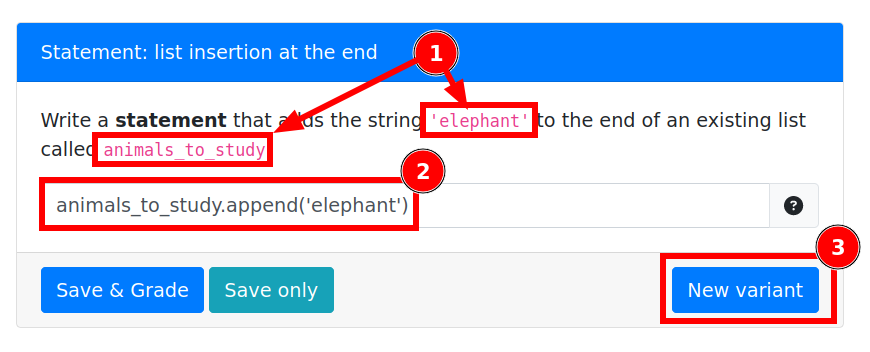
\includegraphics[width=300px]{imgs/pl-question.png}
  \caption{
    An example of a statement question from the course. (1) Elements of these
    questions (e.g., variables, values) are randomized, (2) students are
    expected to write a single line of code using those variables and values to
    accomplish a task, and (3) students can generate new variants of the
    questions allowing for more practice.
  } 
  \label{fig:append-stmnt}
\end{figure}

The construction of our sets of distactor templates begins with a set of
problems we refer to as ``statement questions''. These questions require students
write a single line of code that accomplishes some task such as appending to an
existing list (Figure~\ref{fig:append-stmnt}). Responses to these questions are
much simpler to analyze than typical code writing solutions as they restrict
possible misconceptions and errors to the one particular concept covered by a
given question.  In total, 42 of these questions have been deployed thus far in
the course from which we draw our set of submissions on both homework and exams
with the questions covering the majority of operations relating to the manipuation of 
Pythons builtin data structures. To collect a set of these 
errors for each of these operations we parse all errors into abstract syntax
tree representations of the code. From this, we then engage in an iterative 
process of manually looking for similar groups of errors, constructing a 
partial AST that characterizes that group of error, and filtering those errors
from the corpus of responses. This process is repeated until no more groups of
errors can be identified.  

\begin{figure}[t]
    \centering
    \resizebox{0.5\textwidth}{!}{
        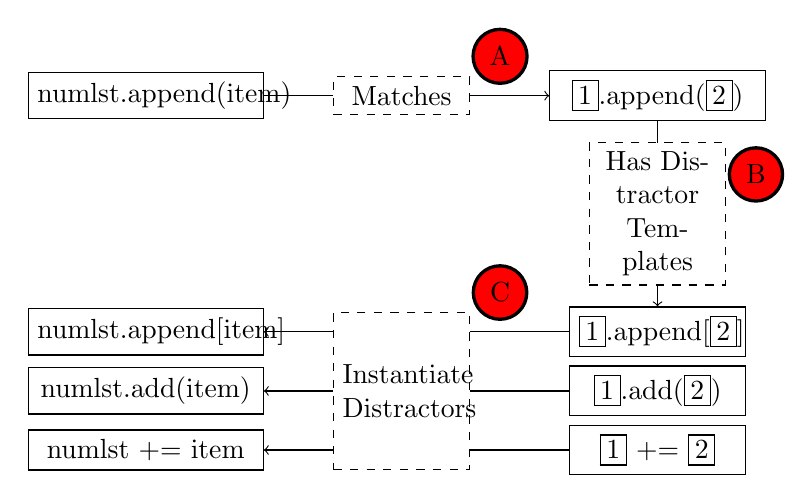
\begin{tikzpicture}[node distance=2cm]

    \node (line) [draw, text width=2.75cm, align=center] {numlst.append(item)};
    \node (extract) [draw, xshift=4.5cm, right of=line, text width=2.5cm, align=center] {\boxed{1}.append(\boxed{2})};

    \node (d1struct) [draw, yshift=-1cm, below of=extract,    text width=2cm, align=center]   {\boxed{1}.append[\boxed{2}]};
    \node (d2struct) [draw, yshift=1.25cm, below of=d1struct, text width=2cm, align=center] {\boxed{1}.add(\boxed{2})};
    \node (d3struct) [draw, yshift=1.25cm, below of=d2struct, text width=2cm, align=center] {\boxed{1} += \boxed{2}};

    \node (d1) [draw, yshift=-1cm, below of=line, text width=2.75cm, align=center] {numlst.append[item]};
    \node (d2) [draw, yshift=1.25cm, below of=d1, text width=2.75cm, align=center]       {numlst.add(item)};
    \node (d3) [draw, yshift=1.25cm, below of=d2, text width=2.75cm, align=center]       {numlst += item};

    % Arrows
    \draw[->] (line.east) -- (extract.west);
    \draw[->] (extract) -- (d1struct);
    \draw[->] (d1struct.west) -- (d1.east);
    \draw[->] (d2struct.west) -- (d2.east);
    \draw[->] (d3struct.west) -- (d3.east);

    % Transition labels
    \node (matches) [fill=white, xshift=1.25cm, right of=line, draw, text width=1.5cm, align=center, dashed] {Matches};
    \node (hasdist) [fill=white, yshift=0.5cm, below of=extract, draw, text width=1.5cm, align=center, dashed] {Has Distractor Templates};
    \node (instantiate) [text centered, fill=white, xshift=-1.25cm, left of=d2struct, draw, text width=1.5cm, minimum height=2cm, dashed] {Instantiate\\ Distractors};

    % Labels
    \node (1) [draw, circle, right of=matches,     fill=red, very thick, xshift=-0.75cm, yshift=0.50cm] {A};
    \node (2) [draw, circle, right of=hasdist,     fill=red, very thick, xshift=-0.75cm, yshift=0.50cm] {B};
    \node (3) [draw, circle, right of=instantiate, fill=red, very thick, xshift=-0.75cm, yshift=1.25cm] {C};


\end{tikzpicture}


    }
    \caption{Transforming \texttt{numlst.append(item)} into a set of distractors.}
    \label{fig:appendastmatchesed}
\end{figure}

To enable the rapid authoring of questions that include distrators, we also 
developed a process of autogenerating distractors for a given, correct piece of code.
This is done by leveraging the errors we discovered through the previously
mentioned analysis process.  The process begins by one again constructing
partial ASTs for the correct form of each of the statements for which sets of
distractor templates were constructed.  For example, if we want to support
creating distractors for the append statement we would construct a partial AST
for \texttt{\boxed{1}.append(\boxed{2})}.  As shown in
Figure~\ref{fig:appendastmatchesed}, if a line of code is then entered that
matches this partial AST (e.g., \texttt{numlst.append(item)}) that match can
(A) be identified and (B) the set of distractor templates associated with the
matched statement can be retrieved. The final step (C) involves extracting and
unparsing the subtrees from the original line of code's AST that are occupied
by wildcards in the partial AST. These subtrees represent the values that will
be placed into their respective positions in the distractor templates in order
to generate the final set of distractors.

With this set of distractors collected and a process for generating them put in
place, we then performed a pilot study aimed at evaluating the impacts of including
distractors in Parsons problems on exams. In doing so, we created three pairs of items
were each pair had the same prompt and base solution but one version contained jumbled
distractors and the other did not. These questions were then randomly assigned to
students on a final exam in a large, introductory Python course.  We then
evaluated these items using the following metrics: 
\begin{enumerate}
    \item \textit{Performance}: Students were allowed three attempts. On each of these attempts, students could earn a maximum of 6, 3, and 1 point respectively. Partial credit within these attempts was calculated using an edit distance approach introduced by \citet{poulsen2022efficient}.
    \item \textit{Duration}: This was calculated as the number of seconds a student spent viewing a question during an exam regardless of whether or not they arrived at a correct response.
    \item \textit{Item Discrimination}: In keeping with the standards of Classical Test Theory, we calculate item discrimination as the Pearson's Correlation between item score and exam score.~\footnote{Multiple choice and true-false questions were omitted from the calculation of total-score as those questions cover topics relating to general computing knowledge rather than programming and show only a modest correlation to those elements of the exam related to programming (e.g., code-writing, tracing)}
\end{enumerate}
Mann-Whitney U tests were used to compare the distractor and non-distractor
versions of each item on each of these metrics.

\paragraph{Results and Takeaways:}

% Make two sub tables for performance and duration


\begin{table}[t]
    \begin{minipage}{0.49\linewidth}
        \centering
        \resizebox{\textwidth}{!}{
        \begin{tabular}{lllllllll}
            & \multicolumn{3}{c}{With Distractors}       & \multicolumn{3}{c}{Without Distractors} &        &        \\ \cline{2-7}
            & N  & Mean               & SD                   & N   & Mean                 & SD     & U      & p        \\ \hline
            P1: Append & 84 & 5.23          & 1.49               & 83 & 5.59             & 1.14 & 3952.0 & $>$0.05\\%0.0582  \\
            P2: Count  & 84 & 3.55          & 2.13               & 82 & 4.25             & 1.93 & 4105.0 & $<$0.05*\\%0.0313* \\
            P3: Remove & 73 & 4.05          & 1.99               & 83 & 4.29             & 1.88 & 3175.5 & $>$0.05\\\hline%0.5977  \\
        \end{tabular}}
        \caption*{Subtable 3a: Results for Performance}
        \label{tab:pp-performance}
    \end{minipage}%
    \hfill
    \begin{minipage}{0.49\linewidth}
        \centering
        \resizebox{\textwidth}{!}{
        \begin{tabular}{lllllllll}
            & \multicolumn{3}{c}{With Distractors}         & \multicolumn{3}{c}{Without Distractors} &        &        \\ \cline{2-7}
            & N  & Mean                & SD                    & N    & Mean                   & SD       & U      & p            \\ \hline
            P1: Append & 84 & 123.05         &  77.33              & 83   &  89.96             & 79.85 & 2057.5 & $<$0.001***\\%4.860e-06*** \\
            P2: Count  & 84 & 271.38         & 174.10              & 82   & 217.75            & 194.66 & 2548.5 & $<$0.01**\\%3.843e-03**  \\
            P3: Remove & 73 & 179.57         & 106.00              & 83   & 156.37            & 156.28 & 2046.0 & $<$0.001***\\ \hline%4.805e-04*** \\
        \end{tabular}}
        \caption*{Subtable 3b: Results for Performance}
        \label{tab:pp-duration}
    \end{minipage}
    \caption{Results of the Mann-Whitney U tests comparing duration and performance on the distractor and non-distractor versions of each item.}
\end{table}

%\begin{table}[t]
%    \centering
%    \begin{tabular}{lllllllll}
%    \hline
%                        & \multicolumn{3}{c}{With Distractors}       & \multicolumn{3}{c}{Without Distractors} &        &        \\ \cline{2-7}
%                        & N  & Mean               & SD                   & N   & Mean                 & SD     & U      & p        \\ \hline
%    P1: Append & 84 & 5.23          & 1.49               & 83 & 5.59             & 1.14 & 3952.0 & $>$0.05\\%0.0582  \\
%    P2: Count  & 84 & 3.55          & 2.13               & 82 & 4.25             & 1.93 & 4105.0 & $<$0.05*\\%0.0313* \\
%    P3: Remove & 73 & 4.05          & 1.99               & 83 & 4.29             & 1.88 & 3175.5 & $>$0.05\\\hline%0.5977  \\ \hline
%    \end{tabular}
%    \caption{Results of the Mann-Whitney U tests comparing performance on the distractor and non-distractor versions of each item.}
%    \label{tab:pp-performance}
%\end{table}
%\begin{table}
%    \begin{tabular}{lllllllll}
%    \hline
%                        & \multicolumn{3}{c}{With Distractors}         & \multicolumn{3}{c}{Without Distractors} &        &        \\ \cline{2-7}
%                        & N  & Mean                & SD                    & N    & Mean                   & SD       & U      & p            \\ \hline
%    P1: Append & 84 & 123.05         &  77.33              & 83   &  89.96             & 79.85 & 2057.5 & $<$0.001***\\%4.860e-06*** \\
%    P2: Count  & 84 & 271.38         & 174.10              & 82   & 217.75            & 194.66 & 2548.5 & $<$0.01**\\%3.843e-03**  \\
%    P3: Remove & 73 & 179.57         & 106.00              & 83   & 156.37            & 156.28 & 2046.0 & $<$0.001***\\ \hline%4.805e-04*** \\ \hline
%    \end{tabular}
%    \caption{Results of the Mann-Whitney U tests comparing duration on the distractor and non-distractor versions of each item.}
%    \label{tab:pp-duration}
%\end{table}}


% Summary of results
The results of the pilot study indicate that the questions with distractors
took significantly longer to complete across all three pairs of questions
(Table~3a) with a low to moderate effect size
($d$=0.17-0.42). Of the three pairs of questions, only one showed a significant
difference in performance with the distractor versions of the questions being
more difficult (Table~3b).  As for item discrimination,
both questions with and without distractors showed high correlations with the
exam score well above the generally accepted threshold of 0.4 which is often
used to define a ``good'' item~\cite{matlock1997basic}. The inclusion of
distractors did not appear to lead to an increase or decrease in item
discrimination that would be considered practically significant.

% Summary of takeaways
Overall, the results of this pilot study draws into question the utility of
including jumbled distractors in Parsons problems on summative assessments.
If the intention of the summative assessment in questions is to reliably
discriminate between high and low performing students the results presented
suggest that the inclusion of jumbled distractors does little to help this
endeavor. In particular, given the large increase in duration seen for the 
distractor versions of the questions, increasing the reliability of the
assessment by including additional Parsons problems which do not include
distractors may be a more effective approach.  However, given this was a pilot
study which included only a small number of questions, these findings motivate
our subsequent, larger scale evaluations of the utility of distractors in
Parsons problems on summative assessments.



\subsection{Evaluating Distractors}\label{sec:parsons}

\paragraph{Abstract:} Since the project described in the previous section we
have performed a number of follow up studies aimed at evaluating the impacts of
including distractors on Parsons problems in summative assessments.  The first
of these, conducted in the Fall of 2021, was a replication of  the pilot study
described in the previous section which took place over the course of a full
semester~\cite{smith2023investigating}. And extension of this work was then
conducted in the Spring of 2022 in which we evaluated the impacts of including
visually grouped distractors on Parsons problems~\cite{smith2023comparing}. 

\paragraph{Methodology:} This study involves a between-subjects, randomized
experiment. Students in the Fall 2022 semester ($n=576$) were randomly assigned
to one of two conditions: jumbled distractors (JD) or no distractors (ND).
Students in the Spring 2023 semester ($n=456$) were randomly assigned to either
the visually grouped distractors (GD) or no distractors (ND) condition. In both
semesters, the ND questions were kept the same and students performance on
those questions did not differ significantly between the two semesters
(t=-1.63, p>0.05). This supports the assumption that the two semesters were
comparable in terms of student performance.


% What was the assessment structure
Each semester included four quizzes and four exams which were unproctored and
proctored, respectively. All quizzes and exams were computer-based, with
quizzes taken on the students' own devices and exams by scheduling a time in a
proctored computer lab~\cite{zilles2019every}. In each semester, 32 question
pairs were used in the exams, and the questions not containing distractors were
kept largely identical throughout both semesters with the exception of two
items pairs which were replaced. 

For determining the impact of including visually grouped and jumbled
distractors on performance and duration, we fit a series of Multi-Level Models
(MLM)~\cite{snijders2011multilevel}. The purpose of using this modeling
approach compared to a more standard linear regression is to help account for
variance that might occur within the conditions (ND, JD, GD) and within student
performance. Importantly, MLMs allows us capture the unobserved variance in the
conditions independent of unobserved variance in student performance, thereby
allowing us to better model when outcomes are more impacted by student
performance or by question.


% First regression - What is the impact of JD and GD relative to no distractors
\noindent \paragraph{Regression Set 1 - Comparing No Distractors to Each Distractor Condition:}
The first regression form is used to determine the impacts of including visually grouped  
and jumbled distractors relative to not including distractors. We fit the
following pair of MLMs.
\begin{align*}
  \text{Performance}_{ij} = \beta_0 +  \beta_1\text{Condition}_{ij} + \beta_{2i}\text{S}_{i} + \text{Q}_{j} + \epsilon_{ij}\\
  \text{Duration}_{ij} = \beta_0 + \beta_1\text{Condition}_{ij} + \beta_{2i}\text{S}_{i} + \text{Q}_{j} + \epsilon_{ij} 
\end{align*}
Here, $\text{Performance}_{ij}$ and $\text{Duration}_{ij}$ are the performance
and duration of student $i$ on question $j$, respectively.
$\text{Condition}_{ij}$ is the condition student $i$ was assigned to for
question $j$ (i.e., ND, JD, GD). $\text{S}_{i}$ is included as a fixed effect
to control for student ability on Parsons problems. $\text{Q}_{j}$ is included
as a random effect to control for question properties (i.e. average performance
or duration on a given question) and to help quantify how much variance in the
model comes from variance between questions versus variance between student
performance within a question.  $\epsilon_{ij}$ is the error term for student
$i$ on question $j$.  Of the coefficients that result from these regressions,
ones that are pertinant to the results are the intercept ($\beta_0$) which is
the average for a given outcome on the ND condition and $\beta_1$ which is
average outcome for each of the remaining two conditions relative to the
intercept. 

\noindent\paragraph{Regression Set 2 - Comparing JD to GD}
To directly compare the impacts of visually grouped and jumbled distractors we fit 
the following second pair of MLMs.
\begin{align*}
  \text{Performance}_{ij} = \beta_0 + \beta_1\text{Distractor}_{ij} + \beta_2\text{Grouped}_{ij} + \beta_{3i}\text{S}_{i} + \text{Q}_{j} + \epsilon_{ij}\\
  \text{Duration}_{ij} = \beta_0 + \beta_1\text{Distractor}_{ij} + \beta_2\text{Grouped}_{ij} + \beta_{3i}\text{S}_{i} + \text{Q}_{j} + \epsilon_{ij} 
\end{align*}
In this model the $\text{Condition}_{ij}$ predictor is replaced with two binary
predictors, $\text{Distractor}_{ij}$ and $\text{Grouped}_{ij}$  indicating if
question $j$ contains distractors and if those distractors are grouped. We
choose to run this second set of models for a more fine-grained comparison,
even though the models are functionally equivalent to the first set. In
particular, reconfiguring the model in this fashion allows us to directly
compare the impact of the JD and GD conditions, as opposed to comparing them
against ND, enabling us to observe whether the differences between the GD and
JD condition are statistically significant. For item-discrimination, we compare the relative impact of including
distractors for each item pair using a paired t-test.

\paragraph{Results and Takeaways:}

\begin{figure*}
  \begin{subfigure}[b]{0.3\textwidth}
    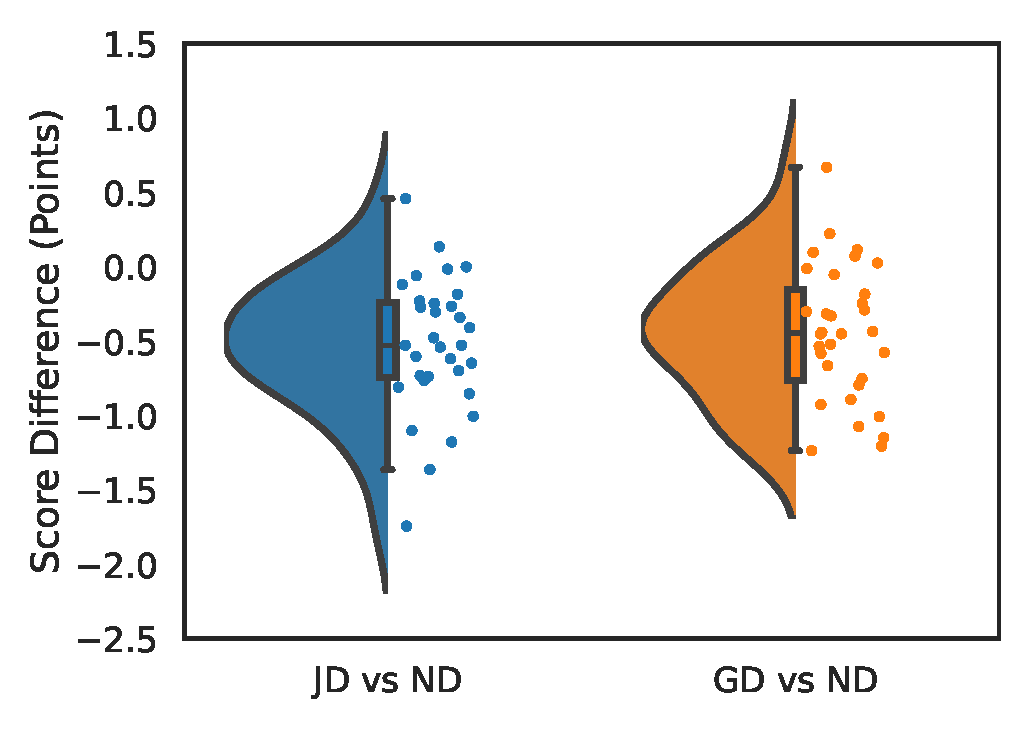
\includegraphics[width=\textwidth]{./imgs/score_dif.pdf}
    \caption{Item Score Comparison}
    \label{fig:score_dif}
  \end{subfigure}%
  \hfill
  \begin{subfigure}[b]{0.3\textwidth}
    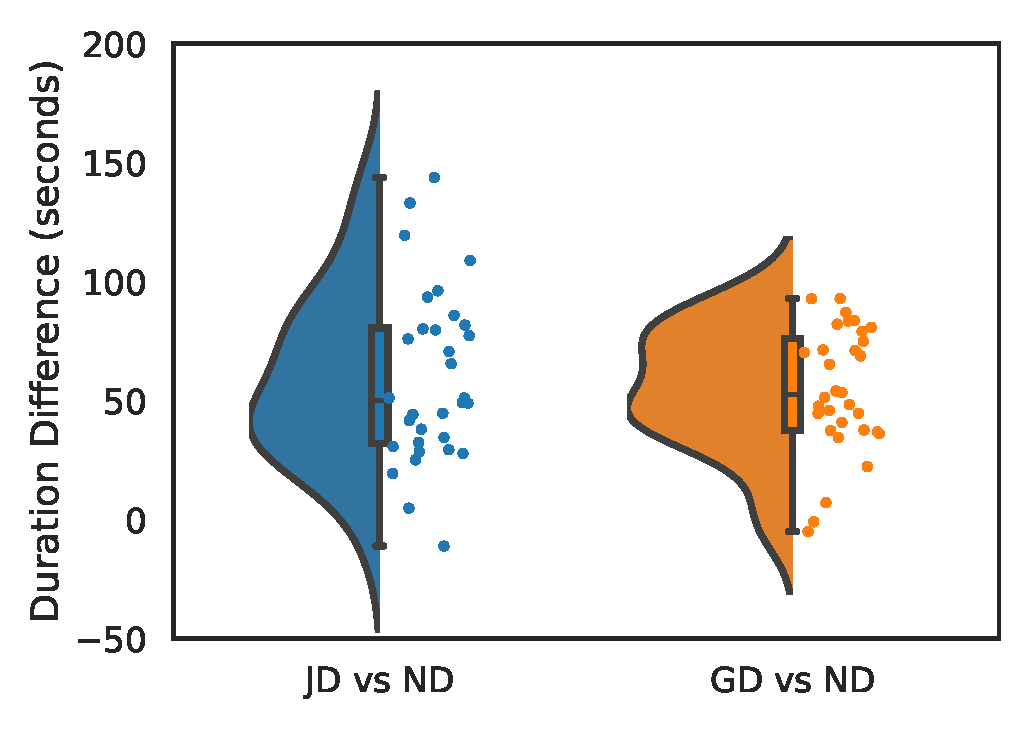
\includegraphics[width=\textwidth]{./imgs/dur_dif.pdf}
    \caption{Item Duration Comparison}
    \label{fig:dur_dif}
  \end{subfigure}%
  \hfill
  \begin{subfigure}[b]{0.30\textwidth}
    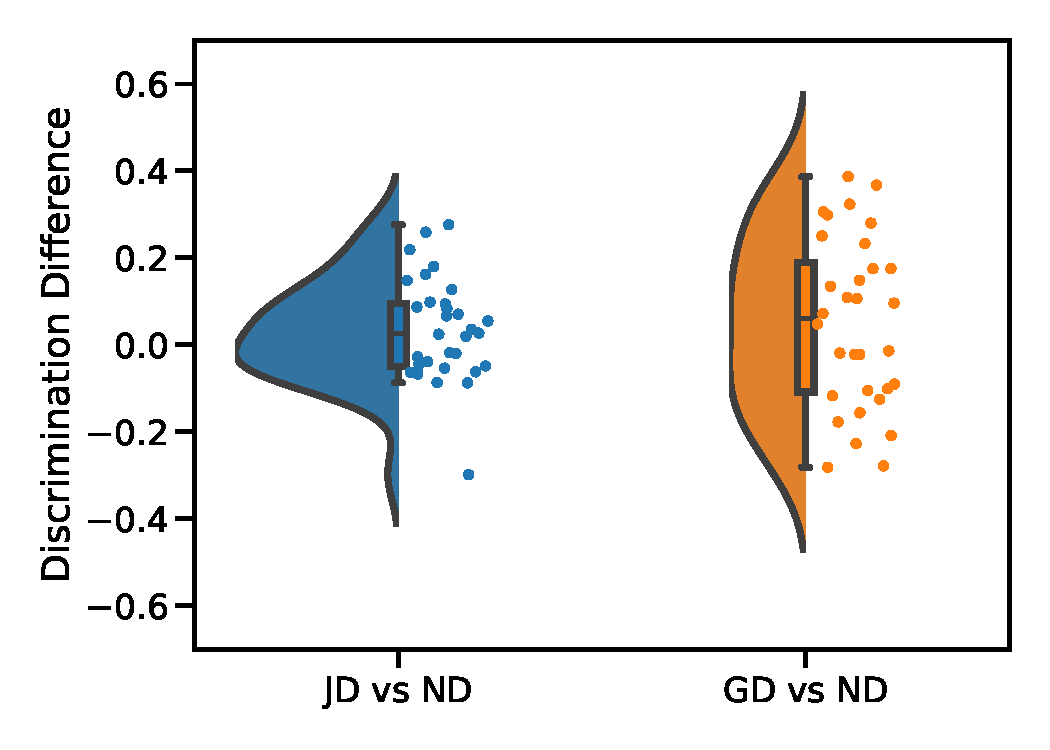
\includegraphics[width=\textwidth]{./imgs/discrim_dif.pdf}
    \caption{Discrimination Comparison}
    \label{fig:discrim_dif}
  \end{subfigure}
  \caption{The item pairs are displayed with the difference in score (Figure~\ref{fig:score_dif}), duration
  (Figure~\ref{fig:dur_dif}), and
  item-discrimination (Figure~\ref{fig:discrim_dif}) between the two items on
  the x axis. This is calculated by subtracting the given measure for the item containing
  distractors (i.e., JD, GD) from the measure of the item not containing
  distractors (ND).}
\end{figure*}

With respect to score, examining the graphs in Figure~\ref{fig:score_dif} we
see that the distribution of difference distribution of score difference between
the JD and ND conditions had a slightly lower median than the distribution of
score difference between the GD and ND conditions. This suggests that including
distractors that are visually grouped might have a slightly lower impact on score
compared to including distractors that are jumbled. Results of the regression
analysis support this indicating that the JD condition was significantly more 
difficult than the ND condition ($\beta = -0.55$, $p = 0.008\text{**}$) while
the GD condition was not ($\beta = -0.22$, $p = 0.28$). However, it is worth
noting that the results of the second regression analysis indicates that the GD
condition did not have a significantly different impact on score than the JD
condition ($\beta = 0.33$, $p = 0.12$).

Both distributions of duration differences in Figure~\ref{fig:dur_dif} indicate
the including distractors, either jumbled or grouped, increased the amount of
time students spent on the problem by just under a minute. Results of the first
regression indicates both the JD ($\beta = 60.7$, $p<0.001\text{***}$) and GD ($\beta
= 44.98$, $p = 0.002\text{**}$) conditions had a significant impact on duration.
However, the GD condition did not have a significantly different impact on
duration than the JD condition ($\beta = -18.7$, $p = 0.20$). The one
noteworthy qualitative difference in the distributions of duration differences
is that the distribution for GD appears to have fewer outliers than the
distribution for JD. This suggests that the GD condition may have been more
consistent in its impact on duration than the JD condition.


Finally, for item-discrimination, Figure~\ref{fig:discrim_dif} indicates that
both distractor conditions were associated with a small increase in item
discrimination relative to the no distractor condition. Additionally, it
appears that the GD condition had a slightly larger impact on item
discrimination than the JD condition.  The results of the t-tests indicate that
in the comparison between ND ($M=0.58,\ SD=0.098$) and JD ($M=0.61,\ SD=0.083$),
there was an increase in discrimination that was not statistically
significant($t=1.42,\ p=0.16$).  The results for the comparison between between
the ND ($M=0.55,\ SD=0.17$) and GD ($M=0.61,\ SD=0.13$) showed a similar increase
however, once again, this increase was not statistically significant ($t=1.24,\
p=0.22$). It is worth noting that the inclusion of distractors did not appear to
have a negative impact on item-discrimination in the aggregate. 

Considering our results, we are inclined to recommend that distractors be
avoided on Parsons problems deployed on exams due to the substantial increase
in duration seen in both the JD and GD conditions. However, the marginal
increase in discrimination and opportunity for diagnosing student difficulties
may make distractors desirable for formative contexts, where increasing
time-on-task and exposing students to a variety of common mistakes could help
them avoid these mistakes in the future. If instructors wish to include
distractors on their exams, particularly to assess skills related to avoiding
distractors, visually grouped distractors appear to be a better choice than
jumbled distractors.


\section{Limitations of Published Work}

The primary limitations of the prior work are threefold. First, the distractors
being used are limited to those that can be generated from the errors students
make on statement questions used in the course. These are primarily limited to
operations used to manipulate Python's builtin data structures. The results of
the prior studies may differ if the distractors used focused on looping and
conditional structures. For example, recent work by
\citet{fromont2023exploring} found that blocks in faded (fill in the blank)
Parsons problems that required students to complete conditionals proved to be
the most difficult.


Secondly, my prior work on using distractors in summative assessments 
failed to account for how the number of distractors groups present in a problem
impacts the results. The majority of problems in the prior studies only
contained either one or two groups of distractors. It may be the case that
a larger number of groups with a more diverse set of distractors leads to 
a more measurable increase in item quality. Conversely, it might also be the
case that by including more distractors the item experiences more ``slip'' 
and thus decreases the item quality. In either case, further investigations
are needed to identify the impacts of increasing the number of distractor 
groups present in a Parsons problem when used in summative assessments.


Finally, my prior work only evaluated the distractors in the context of
summative assessments. Though prior work has certainly indicated that
distractors are used in Parsons problems when they are used as an exam item,
the original intention of Parsons problems was as a exercise
tool~\cite{parsons2006parson} and is often discussed as being used as a method
for transitioning students into writing code. As such, though my prior work
makes tentative steps towards informing the use of distractors in summative
assessments, it leaves open the door for further investigation into the impact
of distractors on learning outcomes when used in formative contexts.

\section{Ongoing and Future Work}

In addressing the limitations of the completed work, we propose three research
directions:
\begin{enumerate}
  \item[RD1)] Developing a more complete taxonomy of distractors from errors
    students make on write code question in support of RD2 and RD3
    (Section~\ref{sec:taxonomy}).
  \item[RD2)] A larger study, over multiple semesters, on the impact of distractors on the psychometric
    properties of Parsons problems as exam items (Section~\ref{sec:itemquality}).
  \item[RD3)] Investigating the impact of distractors on learning outcomes in a
    variety of CS contexts (Section~\ref{sec:impact}).
\end{enumerate}

\subsubsection{RD1) Building a Taxonomy of Distractors for Python}\label{sec:taxonomy}

\paragraph{Overview:} 

% Overall goal
This proposed work stems from the prior work initially described in
Section~\ref{sec:creation}. We will extend the analysis performed on statement
questions to include errors and categories of errors students make on code
writing activities in order to create a more complete set of distractors from
which a more generalized taxonomy will be built.  

% The data we are looking at
In the introductory programming course from which the data for the first paper
detailed in Section~\ref{sec:creation} was attained we have a variety large
quantity of historical data. Though in that analysis we focused on collecting
errors from historical responses to ``statement questions'', the course in
questions also has a wide variety of code writing and code fixing problems.
These problems typically involve writing or fixing a single function,
respectively. 

\paragraph{Methodology:} This process would involve an extension to the
distractor discovery process covered in Section~\ref{sec:creation}. Historical
data for code writing and code fixing questions would be manually analyzed to
identify sets of errors that students make while writing programs and errors
they struggle to correct, respectively. In achieving this goal, a static 
analysis tool would be created to classify and identify the prevalence of 
these errors. These errors would be roughly categorized into: (1) conditional
structure errors, (2) boolean expression errors, (3) function definition
errors, (4) looping errors. Though, further categories may be added as 
the analysis unfolds. 

\paragraph{Expected Outcomes and Timeline:} The primary deliverable of this study will be
the taxonomy and bank of common errors itself. The utility of this is twofold.
First, it can be used as a guidebook for question authoring. Second, it can be
used in future analysis of distractors to guide how they can be used in
summative and formative contexts alike. With respect to summative assessments,
this may take the form of identifying which distractors lead to the greatest
increase in item-discrimination and item-difficulty. As for formative
assessments, future investigations could identify which categories of
distractors are most effective for learning when used in a formative context.
Having completed similar analysis before, I anticipate the construction of the
static analysis tool would take approximately a semester to complete.


\subsubsection{RD2) Investigating the Impact of Distractors on Learning Outcomes in CS1}\label{sec:impact}}

The second research direction will investigate the impact of distractors on
learning outcomes in a CS1 context. This consists of a A-B study comparing the
learning gains of students who practice a concept with Parsons problems that
include distractors versus those who practice using problems that do not
include distractors.  These studies will additionally include a series of
interviews with students completing the problems to determine if the
distractors provide any additional benefit to the students beyond potential
learning gains. The primary research questions for this study are as follows:
\begin{enumerate}
  \item[RQ1)] What impact does practice with Parsons problems that include distractors have on both short and long term learning gains compared to practice on Parsons problems without distractors?
  \item[RQ2)] How do students problem solving strategies differ when using Parsons problems with distractors compared to those without distractors?
  \item[RQ3)] What are students perceptions when comparing practice with Parsons problems which include distractors to those without distractors?
\end{enumerate}

\paragraph{Methodology:} 

% The quantitative portion
To evaluate the research questions listed above we ran and A-B comparing the
learning gains of students practicing with and without distractors.  In both
conditions students began by completing a short reading on a topic they had not
encountered in the course, in this case Pythons sorting functions:
\texttt{list.sort()} and \texttt{sorted()}.  They then completed a survey on
their familiarity with the functions they read about prior to completing the
reading.  Students were then randomly assigned to one of two groups for
practicing the concepts with Parsons problems. One group included problems
which contained distractors and the other had problems which did not.  Each
group completed a total of fourteen problems, seven for each of the two
functions which were taught in the reading. After completing the practice
activity students were given a post test consisting of the following problem
types:
\begin{itemize}
  \item \textbf{Statement Questions}: Two statement problems were given, one for each function, and students were asked to write a single line of code which sorted a given list.
  \item \textbf{Error Identification and Explanation:} Students were shown a piece of code and asked to (1) identify if the code had an error with respect to how it was sorting the function or manipulating the sorted list and (2) explain the error.
  \item \textbf{Code Writing:} Students were given a task that required the sorting of a list and asked to write a function that accomplished that task.
  \item \textbf{Code Fixing:} Students were given a function that contained errors in how a function was sorting a list and asked to correct the function so it performed the task specified by the prompt.
\end{itemize}
A week later, students were invited back for a retention test containing the
same problem types. Regression analysis was used to determine if there was a
significant difference in the learning gains of students who practiced with and
without distractors for both the post and retention tests.


% The qualitative portion.
To evaluate students problem solving approaches and perceptions of questions 
that include distractors we designed another learning activity similar to that
used for the A-B study. Here, student were asked to complete a short reading about
the \texttt{dict.items()} function. They then completed fourteen Parsons problems 
as a practice activity, seven of which contained distractors and the other seven
which did not. These questions were interleaved and arranged according to their
complexity. Students were asked to think aloud while solving the Parsons
problems and then, upon completing the exercises asked a series of reflection questions:
\begin{enumerate}
  \item Whare are your general thoughts in comparing the questions that did and did not include distractors?
  \item How would you compare the two types of Parsons problems in terms of difficulty?
  \item How would you compare the two types of Parsons problems in terms of their value for learning? For instance which would you prefer to practice with when encountering a new concept and why?
  \item Whare are your thoughts on the feedback you encountered when you selected a distractor?
\end{enumerate}
They were then asked to complete a series of error identification, code
writing, and code fixing questions while thinking aloud. The purpose of this
being to see if and how students reflected on the practice activities when
applying what they learned to other questions. Upon completing those questions
students are asked a single follow up question requesting a general 
reflection on the practice activities and how they felt the practice prepared 
them for the post test.  Once these interviews are completed they will then be
automatically transcribed, reviewed, and corrected. Two researchers will
develop a codebook though an inductive coding approach and interrater
reliability will be determined though the use of a third, external coder.

\paragraph{Expected Outcomes:} The purpose of this study is to replicate and
extend the findings of the 2023 ITiCSE working group which found that practice
with distractors had a significant impact on students ability to fix
code~\cite{ericson2023multi}. This study bears three notable differences from
that study: (1) our distractors have a feedback mechanism which explains why a
distractor block is incorrect, (2) we add an additional question type to the
post tests which evaluates a student's ability to identify and explain an
error, and (3) we perform a larger qualitative analysis to identify
\textit{why} any learning gains we observe might be occurring. In doing so, we
aim to identify the impacts of distractors on learning and provide guidance on
the design and delivery of such questions.

\paragraph{Timeline:} The data collection for the quantitative portion of this
study has already been completed and had undergone preliminary analysis. Several 
interviews have been conducted with students with more currently underway. We are 
targeting ICER 2024 for the publication of this work.
 
\subsubsection{RD3) An Extended Analysis of the Impact of Distractors on Exam Items }\label{sec:itemquality}

% make a figure with four subfloats, each showing a different distractor type
% and the number of distractors per group.
\begin{figure*}[t]
  \centering
  \subfloat[No Distractors]{
    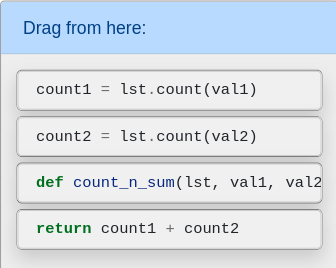
\includegraphics[width=0.24\textwidth]{imgs/rd3_wod.png}
    \label{fig:parsons_no_distractors}
  }
  \subfloat[One Group of Distractors]{
    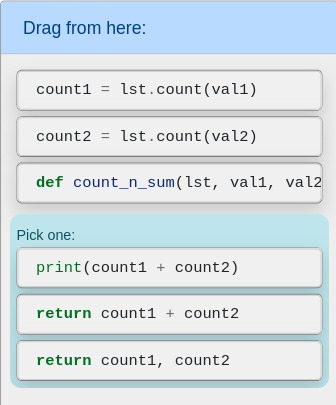
\includegraphics[width=0.24\textwidth]{imgs/rd3_g1.png}
    \label{fig:parsons_onegroup}
  }
  \subfloat[Two Groups of Distractors]{
    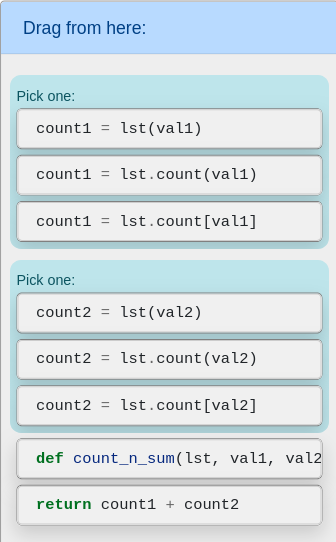
\includegraphics[width=0.24\textwidth]{imgs/rd3_g2.png}
    \label{fig:parsons_twogroups}
  }
  \subfloat[Three Groups of Distractors]{
    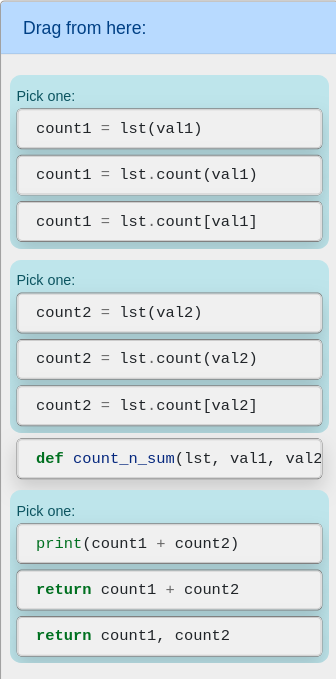
\includegraphics[width=0.24\textwidth]{imgs/rd3_g3.png}
    \label{fig:parsons_threegroups}
  }
  \caption{Four examples of Parsons problems with different numbers of distractor groups.}
  \label{fig:parsonsgroupsrd3}
\end{figure*}

The third and final research direction will involve a long term continuation of
the work described in Section~\ref{eval}. Results from the studies discussed in
that section indicated that the inclusion of distractors had little impact on
the quality of a question from a psychometric perspective while significantly
increasing the amount of time students spent on the questions. Though it is
noteworthy that the inclusion of distractors did not appear to have a negative
impact on the quality of the question, these results do lead to the question of
whether it would be more effective to simply include additional questions on an
exam rather than including distractors in Parsons problems.

A core limitation of this prior work is that it does not consider the impact of
increasing the number of distractor groups in a question. By increasing the 
number of distractor groups it is possible that this will increase the probability
of a student encountering a distractor they find plausible and subsequently
include in their solution. This in turn, may lead to an increase in the
difficulty and discrimination of that question. Additionally, by including 
a greater and more diverse quantity of distractors the results of this study
may give insight into which types of distractors prove most effective. Given
these considerations, we propose the following research questions:
\begin{enumerate}
  \item[RQ1) ] What is the impact of increasing the number of distractor groups on the item-difficulty and item-discrimination statistics of Parsons problem?
  \item[RQ2) ] What is the impact of increasing the number of distractor groups on the amount of time students spend on Parsons problems on exams?
  \item[RQ3) ] How does the effectiveness of distractors vary based on the type of distractor included?
  \item[RQ4) ] How do the results of the above questions differ for each exam taken in the semester?
\end{enumerate}


\paragraph{Methodology:} 

% Experimental Setup
In the Fall 2023 semester we repeated the experiments comparing Parsons
problems with no distractors to those that included jumbled and visually
grouped distractors. In this iteration of the experiment we constructed
problems eight sets of problems. Each set contained four problems containing
zero to three groups of distractors, respectively
(Figure~\ref{fig:parsonsgroupsrd3}). Otherwise, each had the same prompt and
base solution and only differed in the number of distractors which were
included. These questions were randomly assigned to students on exams and
quizzes throughout the semester. 

% IRT and CTT Analysis
We perform CTT and IRT analysis to compare the difficulty and discrimination
based on the number of distractors present in the question. We additionally use
the estimated viewing times on PrairieLearn to determine how the amount of time
students spent on the questions differed based on the number of distractors the
Parsons problem contained. This experiment will be run over the next two
semesters in an effort to collect a large and diverse set of problems. In particular,
as IRT models 

% Analysis of Error Types
Looking beyond the item statistics, there is also the question of distractor
effectiveness. In the context of multiple choice questions, distractors are
deemed effective if they are selected by a significant number of students. One
approach to improving multiple choice questions is to iteratively replace
ineffective distractors with more effective ones~\cite{XXX}. In the context of
Parsons problems, we can similarly evaluate the effectiveness of distractors 
and provide guidance on which types of distractors are most effective (e.g.,
boolean expressions, conditional structures, statements). This analysis is 
made possible as a wider variety of distractors are included in the problems
used in this study.

% Differs based on exam
Finally, we will also consider how the results of the above analysis differ
based on the exam in which the questions, and distractors, are included. One 
consideration, particularly with respect to the item analysis, is that including
questions with distractors may have a greater impact on the difficulty and
discrimination of questions on earlier exams in the semester where students
are still gaining familiarity with the basic syntax and semantics of the
language. Similarly, the distractors that prove most effective may differ
based on the point in the semester where students encounter them.

\paragraph{Expected Outcomes:} My prior work on this topic has indicated that 
the inclusion of distractors in Parsons problems has little impact on the
quality of a Parsons problem from a measurement perspective. Those results
were limited in that they did not consider the impact of increasing the number
of distractor groups in a question, which distractors were most effective, or
how the results of this analysis differed based on the exam in which the
questions were included. This study aims to provide a more complete picture of
the impact of distractors on the quality of Parsons problems towards informing
the design of Parsons problems when they are used in summative assessments.

\paragraph{Current Progress and Timeline:} The first set of questions have been 
administered to students in the Fall 2023 semester and preliminary data analysis 
is underway. The data collection for this study will continue through the Spring
2024 semester. I am currently targeting SIGCSE 2025 for the publication of this
work.


\bibliographystyle{ACM-Reference-Format}
\balance
\bibliography{acmart}

\end{document}
\endinput
